\section{Криволинейные интегралы первого рода}
\subsection{Задача о вычислении массы нити}
Пусть есть некоторая тяжелая нить, т.е. кривая AB, обладающая массой.
Пусть кривая спрямляемая и нам известна масса любого кусочка кривой AB.
Т.е. если возьмем точку $M \in AB$, тогда:

\begin{wrapfigure}{r}[5pt]{0.4\textwidth}
\centering 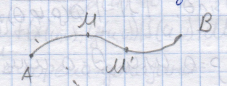
\includegraphics[scale=1]{im.png}
\end{wrapfigure}

Если нить однородна, т.е массы кусочков кривой одинаковой длинны равны,
по отношению массы нити к длине, т.е масса нити единичной длинны называется плотностью

Если нить не однородна, то назовем средней плотностью участка MM' отношение массы участка MM' к
длине MM' $(\frac{\triangle m}{\triangle l})$.
Если $\exists(\lim\limits_{\triangle l \rightarrow 0}\frac{\triangle m}{\triangle l} = A)[A \rightarrow \inf]$, то величина A - это плотность нити в точке $M (\varrho (M) )$.

Пусть известнна плотность нити в каждой точке $(\varrho (M) )$ и нужно определить ее массу.
Для этого разобъем кривую AB точками ${A_i}_{i=0}^{n}\max$,
что $A_0 = A, A_n = B$, причем плотность на отрезке $[A_{i-1}; A_i]$ равна плотности
в $A_i(\varrho ([A_{i-1}; A_i] = \varrho (A_i))$.
Тогда масса дуги $A_{i-1}A_i \approx \varrho (A_i)\triangle l_i ,
где \triangle l_i = \triangle l_i = l_{\overset {\smile} {A_{i-1}{A_i}}}$.

Тогда масса всей нити $AB \approx \sum_{i=1}^{n} \varrho (A_i)\triangle l_i$, и ясно,
что чем меньше разбиение, тем меньше ошибка (и значение суммы будет более близким к массе нити).
Если возьмем $\alpha = \max\limits_{1 \lq i \lq n}\triangle l_i$, то за массу нити возьмем $\lim\limits_{\alpha \rightarrow 0} \sum_{i=1}^{n} \varrho (A_i)\triangle l_i$.

Масса нити не зависит от того, какую точку взять начальной, а длина не зависит от концов.




\subsection{Определение криволинейного интеграла первого рода}
\begin{wrapfigure}{r}[5pt]{0.4\textwidth}
	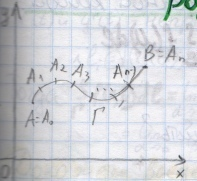
\includegraphics[scale=0.7]{int1.jpg}
\end{wrapfigure}

Пусть в $xOy$ задана спрямляемая кривая, т.е. кривая, у которой есть длина.
И пусть есть функция $f(x,y)$, которая определена на $\Gamma$ (или на Д: Д > $\Gamma$).


Разобъём кривую AB точками $A_i$.
Возьмём $\forall(M;\in \Gamma)$.
Пусть $(\zeta_i;\eta_i )$ --- координаты $M_i$.
Найдем $(\zeta_i;\eta_i )$ и составим сумму: $S_n = \sum^{n}_{i=1} {f(\zeta_i;\eta_i )}_n l_i$

Аналогично можно сделать и в случае если кривая замкнута. Только тогда надо указать начало и направление.

\opred
Если $\exists (\lim\limits_{\alpha \rightarrow 0}(S_n = I) [I \ne 0]$, где $\alpha = \max \triangle l_i$, $S_n = S_n = \sum^{n}_{i=1} {f(\zeta_i;\eta_i )}_n l_i$,
причем I не зависит ни от способа разбиения I на части, ни от выбранных точек $M_i$, то I --- это криволинейный интеграл от $f(x,y)$, взятый по кривой $\Gamma$.
\opred


$$ I = \int\limits_{\Gamma}f(x,y)dxdy = \int\limits_{\Gamma}f(M)dl$$.


Если вернуться к массе нити, то очевидно, что $m=\int\limits{AB}\varrho(M)dl$.

Аналогично можно рассматривать интеграл и по пространственной кривой:

\begin{wrapfigure}{r}[5pt]{0.4\textwidth}
	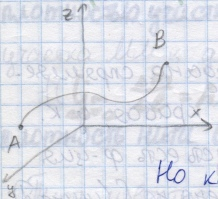
\includegraphics[scale=0.7]{int2.jpg}
\end{wrapfigure}

$\int\limits_{AB}f(x,y,z)dl = \int\limits_{AB}f(M)dl$.


\subsection{Сведение криволинейного интеграла первого рода к обыкновенному определённому интегралу}

\subsubsection{12.1.3 Сведение криволинейных интегралов первого рода к интегралам Римана.}

Пусть в $xOy$ задана непрерывная спрямляемая кривая $\Gamma$.
Предположим, что у нее есть длинна и она параметризована: $y=y(t), x=x(t), t \in [t_0; T]$, причем $A=(x(t_0)y(t_0)), B=(x(T)y(T))$.
Будем считать, что кривая гладкая: $x^{'} (t) и y^{'} (t)$ --- непрерывны (т.е. сами $x(t) и y(t)$ --- непрерывно дифференцируемы).

Пусть есть функция $f(x,y)$, область определения которой содержит кривую $\Gamma$ или равна ей.

$$ \int_\Gamma f(x,y)dl = \lim\limits_{\alpha \rightarrow 0} \sum^{n}_{i=1}{f(\zeta_i;\eta_i )}\triangle l_i $$


Пусть AB разбита точками $A_i = (x(t_i)y(t_i))$.
Обозначим $\zeta_i = (x(\tau_i)), \eta_i = y(\tau_i), f(\zeta_i, \eta_i) = f(x(\tau_i), (y(\tau_i)), \tau_i \in [t_{i-1}; t_i]$.

$$\triangle l_i = \int_{AB}^{t_i}\sqrt{(x^{'}(t))^2 + (y^{'}(t))^{2}}dt$$.


$x^{'}(t) и y^{'}(t)$ --- непрерывны $\Rightarrow$ по теореме о среднем($\int_{a}^{b} f(x) dx = f(M)(b-a), M \in [a;b]$):


$$\triangle l_i = \sqrt {(x^{'}(\Theta_i))^{'} + (y^{'}(\Theta_i)^{2})} \triangle t_i , \triangle t_i = t_i - t_i-1 , \theta_i \in [t_i-1 ; t_i].$$


Тогда $\int_\Gamma f(x,y)dl = \lim\limits_{\alpha \rightarrow 0}\sum^{n}_{i=1}
{f(x(\tau_i), (y(\tau_i))}\sqrt {(x^{'}(\Theta_i))^{2} + (y^{'}(\Theta_i)^{2})}\triangle t_i =
\lim\limits_{\alpha \rightarrow 0}\sum_1 = \int_{t_0}^{T} f(x (t), y(t)) \sqrt {(x^{'}(t))^{2} + (y^{'}(t)^{2})}dt$


Мы знаем, что $\lim\limits_{\alpha \rightarrow 0}\sum^{n}_{i=1}{f(x(\tau_i),
(y(\tau_i))}\sqrt {(x^{'}(\Theta_i))^{2} + (y^{'}(\Theta_i)^{2})}\triangle t_i = 
\lim\limits_{\alpha \rightarrow 0}\sum_1 = 
\int_{t_0}^{T} f(x (t), y(t)) \sqrt {(x^{'}(t))^{2} + (y^{'}(t)^{2})}dt$ --- по определению.
Однако у нас подкоренные функции зависят от $\Theta_i$, а не от $\theta_i$.
Пусть $f(x,y)$ --- непрерывна и $M=sup |f(x,y)|$
Рассмотрим $ \sum^{n}_{i=1}{f(x(\tau_i), (y(\tau_i))}\sqrt {(x^{'}(\tau_i))^{2} + (y^{'}(\tau_i)^{2})}\triangle t_i - \sum^{n}_{i=1}{f(x(\tau_i), (y(\tau_i))}\sqrt {(x^{'}(\Theta_i)){^2} + (y^{'}(\Theta_i)^{2})}\triangle t_i
\le \sum^{n}_{i=1}{f(x(\tau_i), (y(\tau_i))}((\sqrt {(x^{'}(\tau_i))^{2} + (y^{'}(\tau_i)^{2})}) - (\sqrt {(x^{'}(\Theta_i))^{2} + (y^{'}(\Theta_i)^{2})}))\triangle t_i
\le M\sum^{n}_{i=1}{((\sqrt {(x^{'}(\tau_i))^{2} + (y^{'}(\tau_i)^{2})}) - (\sqrt {(x^{'}(\Theta_i))^{2} + (y^{'}(\Theta_i)^{2})}))\triangle t_i}$

Так как $x^{'} и y^{'}$ --- непрерывны, а $\Theta и \tau_i \in [t_i-1; t_i]$ то по следствию из теоремы Кантора:

$\forall (\epsilon > 0)\exists(\beta > 0)\forall(разбиения отрезка [t_0] с диаметром d)[d < \beta \Rightarrow \omega (f) < \epsilon]$ 

т.е $\lim\limits_{\alpha \rightarrow 0}\omega(f)=0$.

$\le M\sum^{n}_{i=1}{\omega(\sqrt {(x^p{'}(\tau_i))^{2} + (y^{'}(\tau_i)^{2})})})\triangle t \underset{\alpha\rightarrow 0}{\rightarrow} 0$.

Таким образом:
$ \mid \sum_1 - \sum_2 \mid \rightarrow 0 \Rightarrow \lim\limits_{\alpha \rightarrow 0}\sum_1 = \lim\limits_{\alpha \rightarrow 0}\sum_2
\Rightarrow \int_\Gamma f(x,y)dl = \lim\limits{\alpha \rightarrow 0}\sum_2 = \lim\limits{\alpha \rightarrow 0}\sum_1 = \int_{t_0}^{T} f(x (t), y(t))(\sqrt {(x^{'}(\tau_i))^{2} + (y^{'}(\tau_i)^{2})}dt$ --- формула сводящая криволинейные интегралы первого рода к интегралам Римана.

Заметим, что для этой формулы даже не нужно условие непрерывности функции $f(x,y)$. Достаточно лишь существования $M=\sup|f(x,y)|$.

Если кривая задана явным уравнением $y=y(x), x \in [a;b], y(x)$ --- непрерывно дифференцируема, то
$$ \int_\Gamma f(x,y)dl = \int_{a}^{b} f(x, y(x))\sqrt{1+(y^{'} (x))^{2}}dx$$

В случае кусочно-гладкой кривой $\Gamma$ криволинейный интеграл по кривой определяется как сумма криволинейных интегралов по всем гладким кривым, составляющим
$\Gamma: \int_\Gamma = \sum^{n}_{i=1} { \int_\Gamma} \Gamma = \overset{n}{\underset{i=1}{\bigcup}} \Gamma_i$

Аналогично --- для пространственной $\Gamma$:
$x=x(t), y=y(t), z=z(t), t\in [t_0, T], \Gamma = AB$,

$ A = (x(t_0)), y(t_0), z(t_0)), B=(x(T), y(T), z(T))$.

$$\int_\Gamma f(x,y,z)dl = \int_{t_0}^{T} f(x(t),y(t), z(t))\sqrt {(x^{'}(t))^{2} + (y^{'}(t)^{2}) + (z^{'}(t)^{2})}dt.$$

Доказательство --- аналогичное двумерному случаю.

Можно рассматривать обобщение криволинейного интеграла на случай кривой заданной в  параметрическом пространстве n штуками уравнений:
$x_i=x_i(t), i=1,n$, причем $x_i(t)$ --- непрерывно дифференцируемы, $f(x_1, ... , x_n)$ - скалярная функция от n переменных, причем:
$ A= (x_1(t_0)), ... , x_n(t_0)), B= (x_1(T), ... , x_n(T)), f:\mathbb{R}^{n} \rightarrow \mathbb{R}^1$.

Если предположить, что $f(x_1, ... , x_n)$ непрерывна на $\Gamma$, то:

$$\int_\Gamma f(x_1, ... , x_n)dl=\int_{t_0}^{T} f(x_1(t), ... , x_n(t))\sqrt {(x_1^{'}(t))^{2} + ... (x_n^{'}(t)^{2})}dt.$$




...

\section{Криволинейные интегралы второго рода}
\subsection{Задача о вычислении работы}
\subsection{Определение криволинейного интеграла второго рода}
\subsection{Сведение криволинейного интеграла второго рода к обыкновенному определённому интегралу}
\subsection{Обобщение на $n$-мерный случай}
\subsection{Связь между криволинейными интегралами первого и второго рода}
\subsection{Ориентация кривой}
\subsection{Формула Грина. Нахождение площади плоской фигуры}
\subsection{Криволинейные интегралы второго рода, не зависящие от пути интегрирования}
...

\section{Элементы теории поверхностей}
\subsection{Понятие поверхности}
\opred

Область - открытое связное множество.

\opred

$G_1$ и $G_2$ - гомеоморфны, если существует взаимооднозначное и взаимонепрерывное отображение одного множества на другое $(f: G_1 \rightarrow G_2)$.

\opred

$f$ - диффеоморфизм класса $C^k$, если $f: G_1 \rightarrow G_2$, где $G_1$ и $G_2$ - гомеоморфны и $f$, $f^-1$ имеют непрерывные производные до порядка $k$ включительно в некоторых открытых можествах, содержащих $G_1$ и $G_2$.

\opred

Понятие поверхности.

Пусть $U$ - область на плоскости с координатами $(u,v)$, ограниченная гладкой, самонепересекающийся, замкнутой кривой.

Непрерывно дифференцируемое отображение $f: \overline{U} \rightarrow \mathbb {R}^3$ такое, что $\frac{D(f^i, f^s)}{D(u,v)} \neq 0$ на всем $\overline{U}$, где $i,s = 1,2,3$ $i<s$, называется гладкая поверхность $S \in \mathbb {R}^3$.

\begin{equation*}
 \begin{cases}
   x = f^1(u,v) 
   \\
   y = f^2(u,v)
   \\
   z = f^3(u,v).
 \end{cases}
\end{equation*}

Это параметрический способ задания поверхности с параметрами $(u,v)$.

Пусть $U_1$ - некоторая гладкая область на плоскости $(u_1,v_1)$ и $S_1$ - гладкая поверхность, которая определяется непредельным дифференцируемым отображением $g: \overline{U_1} \rightarrow \mathbb {R}^3$.

\opred

$S$ и $S_1$ - тождественные, если существует непрерывно дифференцируемый геоморфизм $\varphi: \overline{U_1} \rightarrow \overline{U}$ 
\\
$[f \circ \varphi = g]$, т.е. $\forall i=\overline{1},\overline{3}[f^i(\varphi^1(u_1,v_1),\varphi^2(u_1,v_1)) = g^i(u_1,v_1)]$ и 
\\
$\forall((u_1, v_1) \in \overline{U_1})[\frac{D(\varphi_1, \varphi_2)}{D(u_1,v_1)} \neq 0]$

В этом случае отображения $а: \overline{U} \rightarrow \mathbb {R}^3$ и $g: \overline{U_1} \rightarrow \mathbb {R}^3$ называются различными параметризациями одной поверхности.

\opred

Если $f$ $k$ раз непрерывно дифференцируема, то говорят, что поверхность определяемая этим отображением принадлежит классу $C^k$. 
\\
Тогда переход от одной гладкой параметризации к другой должен осуществляться с помощью диффеоморфизма класса $C^k$.

\opred

Если $f$ не взаимнооднозначно т.е. $\exists (A_1 \neq A_2 : A_1, A_2 \subset \overline{U})[f(A_1) = f(A_2)]$, тогда точка $f(A_1)$ называется кратной.

\opred

Если в качестве пространства параметров взять $(x,y)$, тогда поверхность задается системой:

\begin{equation*}
 \begin{cases}
   x =x 
   \\
   y = y
   \\
   z = z(x,y).
 \end{cases}
\end{equation*}

И такая поверхность называется явно заданная.

\opred

Если есть уравнение $F(x,y,z)=0$, где $F$ - непрерывно дифференцируемо в непрерывной области $(x,y,z)$, тогда совокупность точек $(x,y,z) : F(x,y,z)=0$, называется поверхность, заданная неявно.

\opred

Если в некоторой точке $(x_0,y_0,z_0)$ $F$ удовлетворяет теореме о неявной функции, то часть поверхности в некоторой окрестности этой точки допускает явное представление.
\\
Тогда поверхность заданная неявно, локально сводится к поверхности заданной явно.

Поверхность можно задать в векторном виде:

$\left\{
  \begin{array}{ccc}
x = x(u,v) 
\\
y = y(u,v) 
\\
z = z(u,v) 
  \end{array}
\right.$
$\Rightarrow r = $
$\left(
  \begin{array}{ccc}
x 
\\
y 
\\
z 
  \end{array}
\right)
$
$=$
$\left(
  \begin{array}{ccc}
x(u,v) 
\\
y(u,v) 
\\
z(u,v) 
  \end{array}
\right)$
$= r(u,v)$.
\subsection{Касательная плоскость и нормаль к поверхности}
Пусть $S$ - непрерывно дифференцируемая поверхность. Рассмотрим векторное представление $r = \overline{r}(u,v)$, $(u,v) \in \overline{U}$,
\\
где $r$ - непредельная дифференцируемая векторная функция на $\overline{U}$.

Предположим, что для прямых $u=u_0$ или $v=v_0$, $\overline{U} \bigcap u$ $(\overline{U} \bigcap v)$ состоит из одного отрезка (может быть вырождающейся точкой).

\opred

При сделанных предположениях и при фиксированных $u_0$ или $v_0$, отображение $r$ называется координатная линия:
\\
$r = \overline{r}(u_0,v)$ - $v$ линия,
\\
$r = \overline{r}(u,v_0)$ - $u$ линия.

\opred

$\overline{r_v} = \frac{dr}{dv}$ и $\overline{r_u} = \frac{dr}{dг}$ - касательные вектора.

\opred

Точка поверхности $S$, в которой векторы $\overline{r_u}$ и $\overline{r_v}$ неколлинеарны, называется неособая точка при данной представлении этой поверхности. 

Условие неколлинеарности векторов:
\\
$\overline{r_u} \cdot \overline{r_v} \neq 0$, если точка неособая, то, в частности $\overline{r_u} \neq 0$ и $\overline{r_v} \neq 0$.

\opred

Если $\overline{r_u}$ и $\overline{r_v}$ коллинеарны, то точка называется особая при данном ее представлении.

Рассмотрим кривую на поверхности $S$. Пусть эта кривая задана представлениями $r=r(u(t),v(t))$ где $t \in [t_o, T]$, а $u(t),v(t)$ - непрерывно дифференцируемы, причем $(u'(t))^2+(v'(t))^2 \neq 0$. Тогда 

$$d\overline{r} = \overline{r_u}du+ \overline{r_v}dv = (\overline{r_u}u_t' + \overline{r_v}v_t')dt$$.

\opred

Если точка поверхности неособая, то $dr$ будет касательной к кривой $F(u(t),v(t))$.

\opred

Плоскость, проходящая через точку $\overline{r}(u_0,v_0)$ поверхности, в которой лежат все касательные к кривым $\overline{r}(u(t),v(t))$, проходящим через эту точку, 
\\
называются касательной плоскостью, проходящей через точку $\overline{r}(u_0,v_0)$,
\\
называемую точкой касания.

Если точка неособая, то в ней существует единственная касательная плоскость. Это будет плоскость проходящая через эту точку параллельно векторам $\overline{r_u}(u_0,v_0)$, $\overline{r_v}(u_0,v_0)$.

Уравнение касательной плоскости.

Пусть $\overline{r_0}$ - радиус вектор точки касания, $\overline{r}$ - текущий вектор.
\\
Вектор $\overline{r} - \overline{r_0}$ лежит в плоскости касания и в этой же плоскости лежат вектора $\overline{r_u}$,  $\overline{r_v}$, т.е. $\overline{r_u}$,  $\overline{r_v}$, $\overline{r} - \overline{r_0}$ - компланарны.

Пусть $\overline{r} = (x,y,z)$, $\overline{r_0} = (x_0,y_0,z_0)$. Тогда:
\\
$\left|
  \begin{array}{ccc}
x - x_0 \quad y - y_0 \quad z - z_0
\\
x_u' \quad \quad \quad y_u' \quad \quad \quad z_u'
\\
x_v' \quad  \quad \quad y_v' \quad \quad \quad z_v'
  \end{array}
\right|$
$=$
\\
$=(x-x_0)$
$\left| 
  \begin{array}{ccc}
y_u' \quad z_u'
\\
y_v' \quad z_v'
  \end{array}
\right|$
$+(y-y_0)$
$\left| 
  \begin{array}{ccc}
z_u' \quad x_u'
\\
z_v' \quad x_v'
  \end{array}
\right|$
$+(z-z_0)$
$\left| 
  \begin{array}{ccc}
x_u' \quad y_u'
\\
x_v' \quad y_v'
  \end{array}
\right|$
\\
Если поверхность задана явно, т.е. $z = z(x,y)$, то:
\\
$(x-x_0)$
$\left| 
  \begin{array}{ccc}
0 \quad z_x'
\\
1 \quad z_y'
  \end{array}
\right|$
$+(y-y_0)$
$\left| 
  \begin{array}{ccc}
z_x' \quad 0
\\
z_y' \quad 1
  \end{array}
\right|$
$+(z-z_0)$
$\left| 
  \begin{array}{ccc}
1 \quad 0
\\
0 \quad 1
  \end{array}
\right|$
$=0$

$$z-z_0 = (x-x_0)z_x' + (y-y_0)z_y'$$
\\
Если поверхность задана неявно, т.е. $F(x,y,z) = 0$, то: 

$$(x-x_0)F_x' + (y-y_0)F_y' + (z-z_0)F_z' = 0$$

\opred

Прямая проходящая через точку касания поверхности с касательной плоскостью, перпендикулярная этой плоскости, называется нормальной прямой $K$ поверхности в указанной точке.

Уравнение нормальной прямой 
\\
Пусть $(x_0,y_0,z_0)$ - точка касания. $\overline{r_u}$,  $\overline{r_v}$ лежат в касательной плоскости $K$.
\\
$\overline {n} = [\overline{r_u},  \overline{r_v}] \Rightarrow \overline {n} \bot \overline{r_u}, \overline {n} \bot \overline{r_v} \Rightarrow \overline {n} \bot  K  \Rightarrow \overline {n}$ - нормальный вектор.
\\
$[\overline{r_u},  \overline{r_v}] =$
$\left| 
  \begin{array}{ccc}
i \quad j \quad k
\\
x_u' \quad y_u' \quad z_u'
\\
x_v' \quad y_v' \quad z_v'
  \end{array}
\right|$
$=(y_u'z_v' - y_v'z_u'; x_v'z_u' - x_u'z_v'; x_u'y_v' - x_v'y_u') = \overline{n} $.
\\
Значит, нормальная прямая будет выглядеть так:

$$\frac {x-x_0}{y_u'z_v' - y_v'z_u'} = \frac {y-y_0}{x_v'z_u' - x_u'z_v'} =  \frac {z-z_0}{x_u'y_v' - x_v'y_u'}$$

Если поверхность задана явно, т.е. $z = z(x,y)$, то:

$$\frac {x-x_0}{z_x'} = \frac {y-y_0}{z_y'} = -(z - z_0)$$

\opred

Любой ненулевой вектор, коллинеарный нормальной прямой, проходящий через заданную точку поверхности называется нормаль к этой поверхности в данной точке.

\opred

Вектор нормали единичной длины - единичный вектор нормали.

$(\overline{n_e} = \frac {\overline{n}}{|\overline{n}|}; |\overline{n_e}| = 1)$
\\
Если $\overline{n} = (A,B,C)$, то $\overline{r_u} \cdot \overline{r_v} = A\overline{i} + B\overline{j} + C\overline{k}$. Тогда: 

$\pm \overline{n_e} = \frac {A\overline{i}}{\sqrt{A^2 + B^2 + C^2}}+ \frac {B\overline{j}}{\sqrt{A^2 + B^2 + C^2}}+\frac {C\overline{k}}{\sqrt{A^2 + B^2 + C^2}}$
\\
Вектор нормали может быть направлен вверх или вниз. Поэтому в формуле перед $\overline{n_e}$ стоит знак $\pm$/
\\
Если поверхность задана явно $z = z(x,y)$, то:

$\pm \overline{n_e} = \frac {z_x'}{\sqrt{1 + (z_x')^2 +(z_y')^2}}; \frac {z_y'}{\sqrt{1 + (z_x')^2 +(z_y')^2}};\frac {1}{\sqrt{1 + (z_x')^2 +(z_y')^2}}$
\\
Если поверхность задана неявно т.е. $F(x,y,z) = 0$, то:

$\pm \overline{n_e} = \frac {F_x'}{\sqrt{(F_x')^2 +(F_y')^2+(F_z')^2}}; \frac {F_y'}{\sqrt{(F_x')^2 +(F_y')^2+(F_z')^2}};\frac {F_z'}{\sqrt{(F_x')^2 +(F_y')^2+(F_z')^2}}$
\\
Пусть есть $S$ и $S_1$, причем $S$ задано представлением $\overline{r}(u,v)$, а $S_1$ - $\rho(u_1,v_1)$, где $(u,v) \in \overline{U}$, a $(u_1,v_1) \in \overline{U_1}$;

$\varphi : \overline{U} \rightarrow \overline{U_1}$ - непрерывно дифференцируемый гомеоморфизм, причем:

$\Upsilon = \frac {D(\varphi^1,\varphi^2)}{D(u_1,v_1)} \neq 0$.
\\
Поверхности тождественны $\Rightarrow$ $\rho(u_1,v_1) = r(\varphi^1(u_1,v_1),\varphi^2(u_1,v_1))$
\\
Продифференируем по $u_1$ и $v_1$:

$\overline{\rho_{u_1}}= \overline{r_u}(\varphi_{u_1})^1 + \overline{r_v}(\varphi_{v_1})^1 $ ; $\overline{\rho_{v_1}}= \overline{r_u}(\varphi_{v_1})^1 + \overline{r_v}(\varphi_{v_2})^2 $.

Любая пара векторов $(\overline{r_u},\overline{r_v})$ преобразуется в $(\overline{\rho_{u_1}},\overline{rho_{v_1}})$ c помощью матрицы
$\left(
  \begin{array}{ccc}
(\varphi_{u_1})^1 \quad (\varphi_{u_1})^2
\\
(\varphi_{v_1})^1 \quad (\varphi_{v_1})^2
  \end{array}
\right)$.
По условию $\Upsilon \neq 0 \Rightarrow A \neq 0 \Rightarrow$ переход от $(\overline{r_u},\overline{r_v})$ к $(\overline{\rho_{u_1}},\overline{rho_{v_1}})$ происходит с помощью невырожденной линейной системы $\Rightarrow$ для $(u_1,v_1)$ векторы $\rho_{u_1}$ и $\rho_{v_1}$ линейно независимы $\leftrightarrow \overline{r_u},\overline{r_v}$ - линейно независимы $\leftrightarrow \overline{r_u},\overline{r_v}$ - неколлинеарны $\Rightarrow$ точка неособая.
\subsection{Ориентация поверхности}
\opred

Точка $M_0$ поверхности $S$ внутренняя, если существует окрестность точки $M_0$ такая, что множество точек окрестности, не являющихся точками поверхности представляет собой несвязное множество.

\opred

Точки поверхности не являющиеся внутренними - граничные точки поверхности.
\\
Рассмотрим поверхность $S$; $M_0$ - внутренняя точка. Будем считать, что в некоторой внутренней точке $M_0$ гладкой поверхности $S$ выбрано одно из двух направлений нормали.

\opred

Если при обходе вдоль дугового замкнутого контура $\Gamma$, лежащего на $S$ и, не имеющего общих точек с границей этой поверхности, нормаль, непрерывно изменяясь вдоль $\Gamma$, по возвращению в точку $M_0 \in \Gamma$ вернется к первоначальному направлению, то поверхность $S$ - ориентированная (двусторонняя).

Выбор одного из направлений нормали в какой-либо внутренней точке ориентированной поверхности определяет сторону поверхности.
\\
Примеры:
\\
Двусторонние поверхности:
\\
Полусфера, плоскость, эллипсоид, однополосный гиперболоид.
\\
Односторонняя поверхность - лист Мёбиуса.

Пусть $S$ - двусторонняя поверхность (есть направление нормали). Пусть есть две точки $M_0$ и $M_1 \in S$ и гладкий контур $\Gamma_1$, соединяющий их и не пересекающий границы $S$. Тогда при перемещении из одной точки в другую вдоль $\Gamma$, во вторую точку мы придем с тем же самым направлением нормали.

Если, приходя в $M_1$, по двум разным путям $\Gamma_1$ и $\Gamma_2$ мы получили бы разное направление нормали, то это бы привело к тому, что, двигаясь по замкнутому контуру $M_1 \Gamma_1 M_0 \Gamma_2 M_1$, мы бы пришли в $M_1$ с другим направлением нормали, что противоречит условию.

Таким образом, выбор направления нормали в одной точке однозначно определяет выбор направления нормали на всей $S$. 

\opred

Совокупность точек поверхности с приписанными направлениями нормали называется определённой стороной поверхности.

Пусть $S$ - незамкнутая, гладкая двусторонняя поверхность, ограниченная простым контуром. Обозначим определённое направление обхода в качестве "$+$" , если наблюдатель, двигаясь по контуру видит внутреннюю часть поверхности слева. Противоположное направление - "$-$".

Обозначим за $S^+$ сторону поверхности с "$+$" направлением обхода контура, за $S^-$ - сторону с "$-$" направлением обхода контура.

Рассмотрим негладкую поверхность $S$(кубик). 

Разобьем гладкую поверхность $S$ на две части: $S^+$ И $S^-$: сфера - тут все ясно, тор - проблема.

Но мы ограничимся случаями, когда поверхность разделяется с помощью некоторого гладкого контура и указываем в качестве "$+$" ориентации - внешнюю сторону поверхности, а в качестве "$-$" - противоположную.


\section{Площадь поверхности}
\subsection{Вантуз (сапог) Шварца}
\subsection{Определение площади поверхности}
\subsection{Преобразование элемента площади}
...

\section{Поверхностные интегралы первого рода}
\subsection{Определение поверхностного интеграла первого рода}
\subsection{Существование поверхностного интеграла первого рода и сведение его к обыкновенному двойному интегралу}
\subsection{Приложения поверхностных интегралов первого рода}
...

\section{Поверхностные интегралы второго рода}
\subsection{Определение и свойства}
\subsection{Сведение к обыкновенному двойному интегралу}
...


